\documentclass[aspectratio=169,10pt]{beamer}
% =====================================================================
%  Behaviour Planning and Generation for Multi-Robot Systems
%  Based on Large Language Models  --  15-minute conference talk
%
%  Build:  make          -> build/slides.pdf
%          make clean    -> remove aux files
%          make purge    -> remove build/
%
%  Assets:  logo/  UPM, ETSIT, Robolabo  (conference logo: drop it in
%                  logo/ and point \confLogo at it -- missing files are
%                  skipped automatically, so it builds fine without one)
%           figs/  arena.pdf, singlerobot.pdf, success.pdf, rmse.pdf
%                  (same PDFs used in the paper)
%
%  TIMING: every frame carries a \note with its budget. The notes sum
%  to ~14.5 min, leaving slack before the 15-minute bell.
% =====================================================================
\usepackage[utf8]{inputenc}
\usepackage[T1]{fontenc}
\usepackage{helvet}
\renewcommand{\familydefault}{\sfdefault}
\usepackage{graphicx}
\usepackage{tikz}
\usepackage{xcolor}
\usepackage{amsmath}
\usepackage{booktabs}
\usepackage{colortbl}
\usepackage{array}
\usetikzlibrary{positioning,arrows.meta,shapes.geometric,calc,fit,backgrounds,decorations.pathreplacing}

% =====================================================================
%  TALK CONFIGURATION -- edit everything in this block
% =====================================================================

% ---- Institutional colors -------------------------------------------
\definecolor{upmblue}{RGB}{0,51,160}
\definecolor{upmnavy}{RGB}{0,40,85}
\definecolor{upmred}{RGB}{196,39,43}
\definecolor{upmgray}{RGB}{90,90,90}
\definecolor{upmlight}{RGB}{235,240,250}

% ---- Logos ------------------------------------------------------------
% Drop the ICECER logo into logo/ and point \confLogo at it. Until then
% the guards below simply skip it -- the deck still builds.
\newcommand{\confLogo}{logo/icecer_logo.png}                       % <-- add when available
\newcommand{\instLogoA}{logo/LOGOTIPO-leyenda-color-PNG-p.png}     % UPM
\newcommand{\instLogoB}{logo/LOGO_ESCUELA.png}                     % ETSIT
\newcommand{\instLogoC}{logo/robolabo_cover.jpeg}                  % Robolabo

% ---- Talk metadata -----------------------------------------------------
\newcommand{\talkTitleShort}{LLM-based Multi-Robot Behaviour Planning}
\newcommand{\confShortName}{ICECER 2026}                 % <-- check venue short name
\newcommand{\presenterName}{\'Alvaro Guti\'errez}        % <-- change if someone else presents
\newcommand{\presenterEmail}{a.gutierrez@upm.es}         % <-- verify
\newcommand{\presenterWebsite}{www.robolabo.etsit.upm.es}

\title{Hierarchical Behavior Planning for Multi-Robot Systems Based on Large Language Models}
\author{Luc\'ia Petit \and Rafael Sendra-Arranz \and \underline{\presenterName}}
\institute{ETSI Telecomunicaci\'on, Universidad Polit\'ecnica de Madrid}
\date{ICECER 2026 \\ 3 December 2026, Instambul, Turkey}   % <-- fill in dates/city

% =====================================================================
%  THEME -- no need to edit below this line
% =====================================================================

\setbeamercolor{structure}{fg=upmblue}
\setbeamercolor{frametitle}{fg=upmblue}
\setbeamercolor{title}{fg=upmnavy}
\setbeamercolor{itemize item}{fg=upmblue}
\setbeamercolor{itemize subitem}{fg=upmred}
\setbeamercolor{section in toc}{fg=upmnavy}
\setbeamerfont{frametitle}{series=\bfseries,size=\large}
\setbeamertemplate{navigation symbols}{}
\setbeamertemplate{itemize item}{\small\raise0.35ex\hbox{\textbullet}}
\setbeamertemplate{itemize subitem}{\scriptsize\raise0.3ex\hbox{--}}

\setbeamersize{text margin left=0.7cm, text margin right=0.7cm}

\setbeamertemplate{frametitle}{%
  \vskip4pt%
  \begin{beamercolorbox}[wd=\paperwidth,leftskip=0.7cm,rightskip=0.7cm]{frametitle}%
    \usebeamerfont{frametitle}\insertframetitle\par%
    \vskip1pt%
    {\color{upmblue}\rule{\dimexpr\paperwidth-1.4cm\relax}{0.8pt}}%
  \end{beamercolorbox}%
}

\setbeamertemplate{footline}{%
  \hbox{%
    \begin{beamercolorbox}[wd=.82\paperwidth,ht=2.2ex,dp=1ex,leftskip=0.7cm]{}%
      {\color{upmgray}\scriptsize \talkTitleShort\ \textbullet\ \presenterName\ \textbullet\ \confShortName}%
    \end{beamercolorbox}%
    \begin{beamercolorbox}[wd=.18\paperwidth,ht=2.2ex,dp=1ex,rightskip=0.7cm]{}%
      \hfill{\color{upmblue}\scriptsize\insertframenumber\,/\,\inserttotalframenumber}%
    \end{beamercolorbox}%
  }\vskip2pt%
}

\setbeamertemplate{headline}{%
  \vskip4pt%
  \hspace{6pt}\IfFileExists{\confLogo}{\includegraphics[height=0.65cm]{\confLogo}}{}%
  \hfill%
  \IfFileExists{\instLogoA}{\includegraphics[height=0.95cm]{\instLogoA}\hspace{5pt}}{}%
  \IfFileExists{\instLogoB}{\includegraphics[height=0.65cm]{\instLogoB}\hspace{5pt}}{}%
  \IfFileExists{\instLogoC}{\includegraphics[height=0.65cm]{\instLogoC}\hspace{6pt}}{}%
  \vskip4pt%
}

\newcommand{\logoRow}[1][0.9cm]{%
  \IfFileExists{\confLogo}{\includegraphics[height=#1]{\confLogo}\hspace{16pt}}{}%
  \IfFileExists{\instLogoA}{\includegraphics[height=1.15cm]{\instLogoA}\hspace{16pt}}{}%
  \IfFileExists{\instLogoB}{\includegraphics[height=#1]{\instLogoB}\hspace{16pt}}{}%
  \IfFileExists{\instLogoC}{\includegraphics[height=#1]{\instLogoC}}{}%
}

\newcounter{secnum}
\AtBeginSection[]{%
  \stepcounter{secnum}%
  \begin{frame}[plain,noframenumbering]
    \vspace{1.2cm}
    \hspace{1.5cm}%
    
\begin{tikzpicture}[remember picture]
      \node[anchor=west, text=upmblue!25, font=\fontsize{110}{110}\selectfont\bfseries]
        (num) {\arabic{secnum}};
      \node[anchor=west, xshift=1.4cm, text=upmnavy, font=\Large\bfseries]
        at (num.east) (title) {\insertsectionhead};
      \draw[upmblue, line width=1.2pt] (title.south west) --
        ($(title.south east)+(0.5cm,0)$);
      \draw[upmred, line width=1.2pt] (title.south west)+(0,-0.15) --
        +(1.5cm,-0.15);
    \end{tikzpicture}
    \vfill
  \end{frame}
}

\newcommand{\callout}[2][upmblue]{%
  \begin{beamercolorbox}[wd=\linewidth,sep=6pt,rounded=false]{}%
    \color{#1}\small #2%
  \end{beamercolorbox}%
}

\begin{document}

% ================= Slide: Title =================
\begin{frame}[plain,noframenumbering]
  \vspace{0.5cm}
  {\color{upmblue}\rule{\textwidth}{2.2pt}}\\[10pt]
  \begin{center}
  {\LARGE\bfseries\color{upmnavy}\inserttitle}\\[4pt]
  {\large\color{upmgray}\itshape Keeping the language model out of the control loop}\\[6pt]
  {\color{upmred}\rule{3cm}{2pt}}
  \end{center}
  \vspace{8pt}
  \begin{minipage}{0.55\textwidth}
    \small
    Luc\'ia Petit$^{1}$, Rafael Sendra-Arranz$^{2}$, \textbf{\presenterName$^{1}$}\\[6pt]
    {\scriptsize\color{upmgray}
    $^1$ ETSI Telecomunicaci\'on, Universidad Polit\'ecnica de Madrid, Spain\\
    $^2$ Center for Automation and Robotics, CSIC-UPM, Spain}
  \end{minipage}\hfill
  \begin{minipage}{0.4\textwidth}
    \raggedleft
    \small\color{upmnavy}\textbf{Presented by}\\
    \Large\bfseries\presenterName\\
    {\small\color{upmgray} \presenterEmail}
  \end{minipage}\\[10pt]
  {\color{upmblue}\rule{\textwidth}{0.5pt}}\\[1pt]
  {\small\color{upmgray}\textbf{\insertdate}}\\[8pt]
  \begin{center}
    \logoRow
  \end{center}
  \note{20 s. Hook: an LLM can decide what a robot team should do, but it
  thinks in seconds while a robot acts in milliseconds. This talk is about
  where to put the boundary between those two clocks.}
\end{frame}

% ================= Slide: Roadmap =================
\begin{frame}{Roadmap}
  \vspace{0.2cm}
  \begin{center}
  {\large\color{upmgray}\itshape An LLM decides \emph{what} to do; it never decides \emph{how} to move}\\[6pt]
  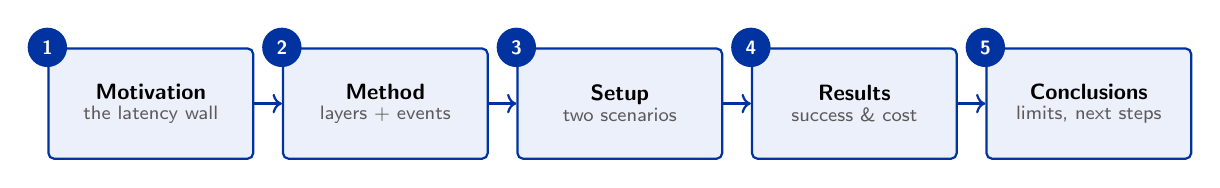
\begin{tikzpicture}[
    every node/.style={font=\footnotesize},
    box/.style={draw=upmblue, thick, rounded corners=2pt, minimum width=2.6cm, minimum height=1.4cm, align=center, fill=upmlight},
    num/.style={circle, fill=upmblue, text=white, font=\bfseries\scriptsize, minimum size=5mm, inner sep=0pt}
  ]
    \node[box] (b1) at (0,0) {\textbf{Motivation}\\[-2pt]{\scriptsize\color{upmgray} the latency wall}};
    \node[box, right=0.35cm of b1] (b2) {\textbf{Method}\\[-2pt]{\scriptsize\color{upmgray} layers + events}};
    \node[box, right=0.35cm of b2] (b3) {\textbf{Setup}\\[-2pt]{\scriptsize\color{upmgray} two scenarios}};
    \node[box, right=0.35cm of b3] (b4) {\textbf{Results}\\[-2pt]{\scriptsize\color{upmgray} success \& cost}};
    \node[box, right=0.35cm of b4] (b5) {\textbf{Conclusions}\\[-2pt]{\scriptsize\color{upmgray} limits, next steps}};
    \node[num] at (b1.north west) {1};
    \node[num] at (b2.north west) {2};
    \node[num] at (b3.north west) {3};
    \node[num] at (b4.north west) {4};
    \node[num] at (b5.north west) {5};
    \draw[upmblue,->,thick] (b1.east) -- (b2.west);
    \draw[upmblue,->,thick] (b2.east) -- (b3.west);
    \draw[upmblue,->,thick] (b3.east) -- (b4.west);
    \draw[upmblue,->,thick] (b4.east) -- (b5.west);
  \end{tikzpicture}
  \end{center}
  \note{25 s. Five parts. The one idea to carry through: deliberation is
  triggered by events, not by the clock.}
\end{frame}

\section{Motivation}

% ================= Coordination: the classical assumption ============
\begin{frame}{Coordinating a robot team}
  \begin{columns}[T]
  \column{0.52\textwidth}
  \textbf{\color{upmnavy}The problem is not locomotion}
  \begin{itemize}
    \item \textbf{Which robot does what, and when}\\[-1pt]
      {\footnotesize\color{upmgray} as the team and the environment evolve}
    \item \textbf{Classical answers are mature}\\[-1pt]
      {\footnotesize\color{upmgray} MRTA as optimisation; self-organised
      threshold and stigmergy schemes}
    \item \textbf{\color{upmblue} Both share one assumption}\\[-1pt]
      {\footnotesize\color{upmgray} the relevant situations are enumerated
      in advance -- as a cost function, or as reactive rules}
  \end{itemize}
  \column{0.48\textwidth}
  \textbf{\color{upmnavy}Where that breaks}\\[4pt]
  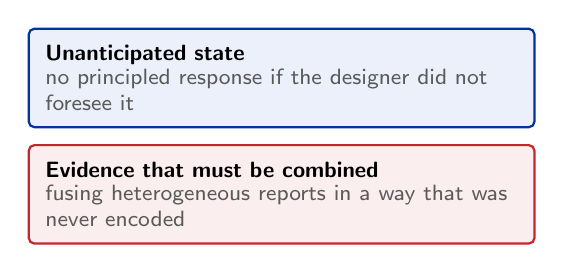
\begin{tikzpicture}[node distance=2mm, every node/.style={font=\footnotesize}]
    \node[draw=upmblue, thick, fill=upmlight, rounded corners=2pt,
          text width=6.0cm, align=left, inner sep=6pt] (c1)
      {\textbf{Unanticipated state}\\[-1pt]
       {\color{upmgray} no principled response if the designer did not
       foresee it}};
    \node[draw=upmred, thick, fill=upmred!8, rounded corners=2pt,
          text width=6.0cm, align=left, inner sep=6pt, below=of c1] (c2)
      {\textbf{Evidence that must be combined}\\[-1pt]
       {\color{upmgray} fusing heterogeneous reports in a way that was
       never encoded}};
  \end{tikzpicture}\\[6pt]
  \callout[upmnavy]{\footnotesize These are exactly the cases where a
  language model could help.}
  \end{columns}
  \note{55 s. Set up the gap: classical MRTA is strong, but only inside
  the space the designer enumerated. Name the two escape cases on the
  right -- they come back in the results.}
\end{frame}

% ================= LLMs + the latency wall ===========================
\begin{frame}{Large language models: the promise and the wall}
  \begin{columns}[T]
  \column{0.5\textwidth}
  \textbf{\color{upmnavy}What they bring}
  \begin{itemize}\small
    \item Reason over a \textbf{symbolic description} of a situation
    \item Ground instructions in feasible skills \textit{(SayCan)}
    \item Interleave reasoning with action \textit{(ReAct)}
    \item Replan from textual feedback \textit{(Inner Monologue)}
  \end{itemize}
  \vspace{2pt}
  \textbf{\color{upmnavy}What they do not bring}
  \begin{itemize}\small
    \item \textbf{\color{upmred}Speed}
  \end{itemize}
  \column{0.5\textwidth}
  \centering
  \textbf{\color{upmnavy}Two clocks, three orders of magnitude apart}\\[6pt]
  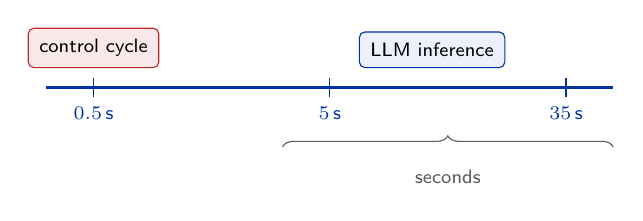
\begin{tikzpicture}[every node/.style={font=\footnotesize}]
    \draw[upmblue, line width=1.1pt] (0,0) -- (7.2,0);
    \foreach \x/\lab in {0.6/$0.5$\,s, 3.6/$5$\,s, 6.6/$35$\,s}
      \draw[upmblue] (\x,0.12) -- (\x,-0.12) node[below, font=\scriptsize]{\lab};
    \node[draw=upmred, fill=upmred!10, rounded corners=2pt, inner sep=4pt,
          anchor=south] at (0.6,0.25) {\scriptsize control cycle};
    \node[draw=upmblue, fill=upmlight, rounded corners=2pt, inner sep=4pt,
          anchor=south] at (4.9,0.25) {\scriptsize LLM inference};
    \draw[decorate, decoration={brace, amplitude=4pt}, upmgray]
      (3.0,-0.75) -- (7.2,-0.75)
      node[midway, below=5pt, font=\scriptsize, color=upmgray]{seconds};
  \end{tikzpicture}\\[10pt]
  \callout[upmred]{\footnotesize\textbf{Any architecture that puts an LLM
  \emph{inside} the control loop inherits this mismatch.}}
  \end{columns}
  \note{60 s. Credit the grounding and closed-loop literature, then land
  the wall: inference is seconds, control is half a second. This is the
  problem the paper attacks.}
\end{frame}

\section{Method}

% ================= Layered architecture ==============================
\begin{frame}{A hierarchical, hybrid architecture}
  \begin{columns}[T]
  \column{0.42\textwidth}
  \vspace{2pt}
  \textbf{\color{upmnavy}Design rules}
  \begin{itemize}\small
    \item \textbf{Two LLM levels}\\[-1pt]
      {\footnotesize\color{upmgray} central allocates macro-tasks;
      per-robot models pick skills}
    \item \textbf{No model below that}\\[-1pt]
      {\footnotesize\color{upmgray} skills and reactive control are plain
      Python}
    \item \textbf{\color{upmblue}The model never emits motor commands}\\[-1pt]
      {\footnotesize\color{upmgray} it can only \emph{name} a skill from a
      closed catalogue}
  \end{itemize}
  \vspace{4pt}
  \callout[upmnavy]{\footnotesize Reasoning where it pays; determinism
  where safety lives.}
  \column{0.58\textwidth}
  \centering
  \resizebox{0.79\linewidth}{!}{%
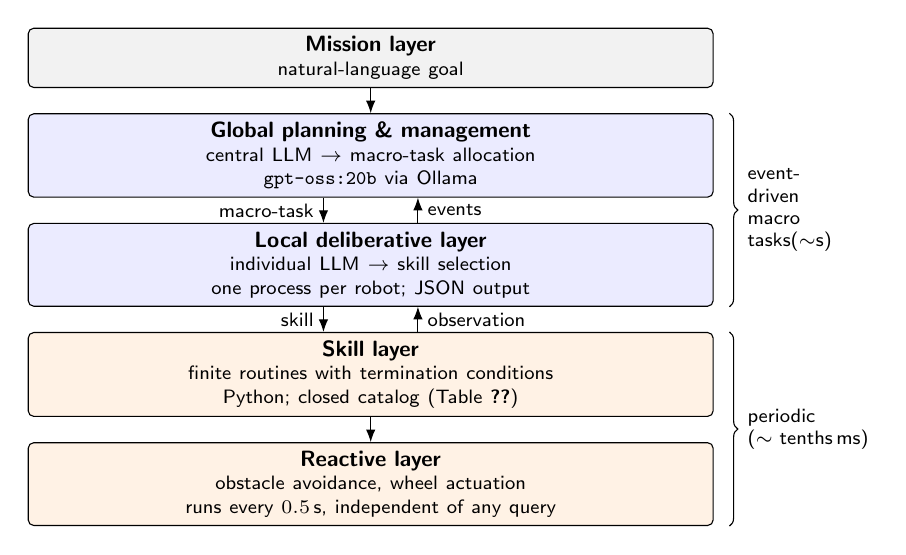
\begin{tikzpicture}[
  font=\footnotesize,
  box/.style={draw, rounded corners=2pt, align=center, inner sep=3pt,
              text width=0.70\columnwidth, minimum height=7.5mm},
  llm/.style={box, fill=blue!8},
  rea/.style={box, fill=orange!10},
  ar/.style={-{Latex[length=1.6mm]}, thin},
]
\node[box, fill=gray!10] (m) {\textbf{Mission layer}\\[-1pt]
  {\scriptsize natural-language goal}};
\node[llm, below=3.2mm of m] (c) {\textbf{Global planning \& management}\\[-1pt]
  {\scriptsize central LLM $\rightarrow$ macro-task allocation}\\[-1pt]
  {\scriptsize{\texttt{gpt-oss:20b} via Ollama}}};
\node[llm, below=3.2mm of c] (l) {\textbf{Local deliberative layer}\\[-1pt]
  {\scriptsize individual LLM $\rightarrow$ skill selection}\\[-1pt]
  {\scriptsize{one process per robot; JSON output}}};
\node[rea, below=3.2mm of l] (s) {\textbf{Skill layer}\\[-1pt]
  {\scriptsize finite routines with termination conditions}\\[-1pt]
  {\scriptsize{Python; closed catalog (Table~\ref{tab:skills})}}};
\node[rea, below=3.2mm of s] (r) {\textbf{Reactive layer}\\[-1pt]
  {\scriptsize obstacle avoidance, wheel actuation}\\[-1pt]
  {\scriptsize{runs every $0.5$\,s, independent of any query}}};

\draw[ar] (m) -- (c);
\draw[ar] ([xshift=-6mm]c.south) -- node[left, pos=0.5, font=\scriptsize]
      {macro-task} ([xshift=-6mm]l.north);
\draw[ar] ([xshift=6mm]l.north) -- node[right, pos=0.5, font=\scriptsize]
      {events} ([xshift=6mm]c.south);
\draw[ar] ([xshift=-6mm]l.south) -- node[left, pos=0.5, font=\scriptsize]
      {skill} ([xshift=-6mm]s.north);
\draw[ar] ([xshift=6mm]s.north) -- node[right, pos=0.5, font=\scriptsize]
      {observation} ([xshift=6mm]l.south);
\draw[ar] (s) -- (r);

\draw[decorate, decoration={brace, amplitude=3pt}]
  ([xshift=2mm]c.north east) -- ([xshift=2mm]l.south east)
  node[midway, right=3pt, font=\scriptsize, align=left]
  {event-\\driven\\ macro\\tasks($\sim$s)};
\draw[decorate, decoration={brace, amplitude=3pt}]
  ([xshift=2mm]s.north east) -- ([xshift=2mm]r.south east)
  node[midway, right=3pt, font=\scriptsize, align=left]
  {periodic\\($\sim$ tenths\,ms)};
\end{tikzpicture}
  }
  \end{columns}
  \note{80 s. Walk top to bottom: mission, central allocation, local skill
  choice, skills, reactive. Then point at the two braces -- blue is
  event-driven in seconds, red is periodic at half a second. That split is
  the contribution.}
\end{frame}

% ================= Bounded action space + self_check =================
\begin{frame}{Bounding what the model can say}
  \begin{columns}[T]
  \column{0.46\textwidth}
  \textbf{\color{upmnavy}Semantic observations}
  \begin{itemize}\small
    \item Raw sensor streams $\rightarrow$ \textbf{discrete, interpretable} state
    \item The model never sees raw arrays
  \end{itemize}
  \vspace{3pt}
  \textbf{\color{upmnavy}Structured output}
  \begin{itemize}\small
    \item JSON: reasoning trace, memory, decision
    \item Central model also restates its own feasibility arithmetic
    \item \textbf{\color{upmblue}Anything outside the catalogue is
      discarded}\\[-1pt]
      {\footnotesize\color{upmgray} robot keeps a safe \texttt{stop};
      last valid behaviour is retained}
  \end{itemize}
  \column{0.54\textwidth}
  \vspace{-2pt}
  {\scriptsize
  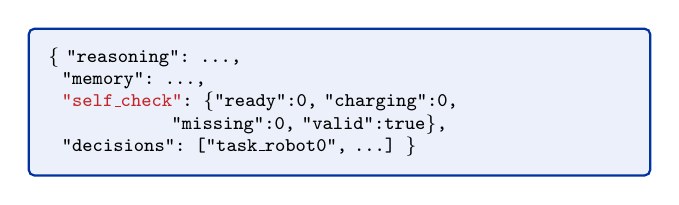
\begin{tikzpicture}
    \node[draw=upmblue, thick, fill=upmlight, rounded corners=2pt,
          inner sep=7pt, text width=7.4cm, align=left, font=\ttfamily\scriptsize]
    {\{ "reasoning": ...,\\
      \ \ "memory": ...,\\
      \ \ \textcolor{upmred}{"self\_check"}: \{"ready":0, "charging":0,\\
      \ \ \ \ \ \ \ \ \ \ \ \ \ \ \ \ \ \ "missing":0, "valid":true\},\\
      \ \ "decisions": ["task\_robot0", ...] \}};
  \end{tikzpicture}}\\[8pt]
  \callout[upmnavy]{\footnotesize Asking the model to \textbf{restate its
  own arithmetic} makes inconsistent assignments detectable without a
  second query.}
  \end{columns}
  \note{55 s. Two guards: the input is abstracted into semantic
  observations, and the output is a closed catalogue plus a self-check
  block. Foreshadow: the self-check is what catches almost every bad
  decision later.}
\end{frame}

% ================= Event-driven synchronisation ======================
\begin{frame}{Event-driven synchronisation}
  \vspace{-2pt}
  \begin{columns}[T]
  \column{0.46\textwidth}
  \textbf{\color{upmnavy}The rule}
  \begin{itemize}\small
    \item Query the model \textbf{only} when the active skill
      \textbf{terminates or fails}
    \item While a query is pending: \texttt{stop} + reactive layer keeps
      the robot safe
    \item Central model queried only at \textbf{coordination moments}\\[-1pt]
      {\footnotesize\color{upmgray} initial planning, recharge completion,
      final aggregation}
    \item Inference in a separate process, shared blackboard\\[-1pt]
      {\footnotesize\color{upmgray} the physics loop never blocks}
  \end{itemize}
  \column{0.54\textwidth}
  \centering
  \textbf{\color{upmnavy}Clock-driven vs.\ event-driven}\\[5pt]
  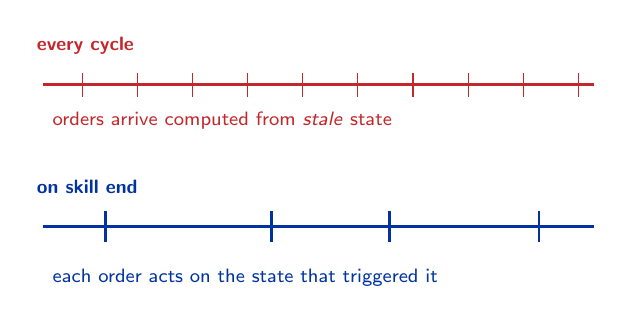
\begin{tikzpicture}[every node/.style={font=\scriptsize}]
    % clock-driven
    \node[anchor=west, color=upmred] at (-0.2,1.5) {\textbf{every cycle}};
    \draw[upmred, line width=1pt] (0,1.0) -- (7.0,1.0);
    \foreach \x in {0.5,1.2,...,6.8}
      \draw[upmred] (\x,1.15) -- (\x,0.85);
    \node[anchor=west, color=upmred, font=\scriptsize] at (0,0.55)
      {orders arrive computed from \emph{stale} state};
    % event-driven
    \node[anchor=west, color=upmblue] at (-0.2,-0.3) {\textbf{on skill end}};
    \draw[upmblue, line width=1pt] (0,-0.8) -- (7.0,-0.8);
    \foreach \x in {0.8,2.9,4.4,6.3}
      \draw[upmblue, line width=1pt] (\x,-0.6) -- (\x,-1.0);
    \node[anchor=west, color=upmblue, font=\scriptsize] at (0,-1.45)
      {each order acts on the state that triggered it};
  \end{tikzpicture}\\[8pt]
  \callout[upmblue]{\footnotesize The model now runs on a time scale
  \textbf{compatible with its own inference cost}.}
  \end{columns}
  \note{65 s. The core slide. Contrast the two timelines: querying every
  cycle guarantees stale orders; tying queries to skill termination makes
  staleness structurally impossible. Next section shows what happens when
  you get this wrong.}
\end{frame}

\section{Experimental setup}

% ================= Platform + scenarios ==============================
\begin{frame}{Platform and scenarios}
  \begin{columns}[T]
  \column{0.37\textwidth}
  \vspace{-2pt}
  \textbf{\color{upmnavy}Platform}
  \begin{itemize}\small
    \item \textbf{Mereli} simulator (ROBOLABO) on \textbf{PyBullet}
    \item e-puck differential-drive robots
    \item $\Delta t = 0.05$\,s; controller $T_s = 0.5$\,s
    \item \textbf{\texttt{gpt-oss:20b}} served \textbf{locally}\\[-1pt]
      {\footnotesize\color{upmgray} Ollama + LangChain, 2$\times$ RTX 2080 Ti}
    \item {\footnotesize\color{upmgray} No external API: latency stays
      under experimental control}
  \end{itemize}
  \vspace{3pt}
  \callout[upmnavy]{\footnotesize \textbf{S1:} 36 runs \quad
  \textbf{S2:} 20 runs $\times$ 5 fleet sizes}
  \column{0.63\textwidth}
  \centering
  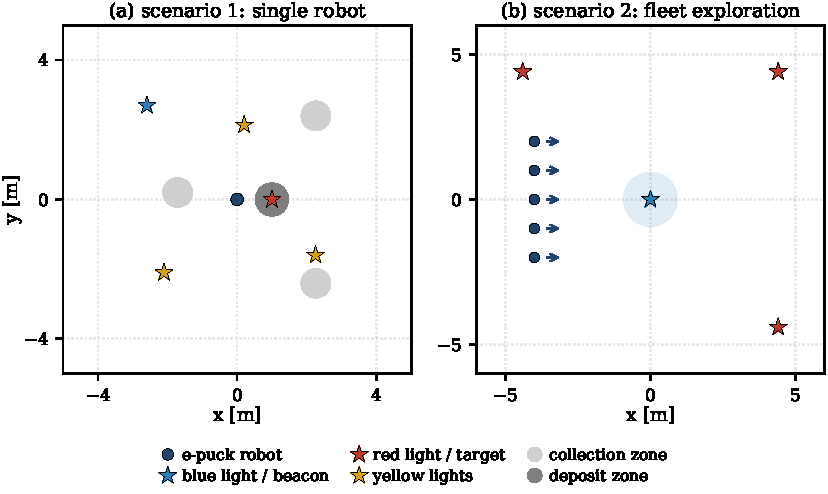
\includegraphics[width=0.90\linewidth]{figs/arena.pdf}\\[2pt]
  {\scriptsize\color{upmgray}
  \textbf{(a)} single robot: forage, recharge two batteries, switch off
  three lights \quad
  \textbf{(b)} fleet: deploy $n$ explorers, detect and localise targets}
  \end{columns}
  \note{55 s. Everything is local inference -- that matters for the
  latency numbers later. Two scenarios: one robot juggling tasks, then a
  fleet doing cooperative exploration.}
\end{frame}

\section{Results}

% ================= Scenario 1 + stale decision walkthrough ===========
\begin{frame}{Scenario 1: why the control loop is the wrong place}
  \vspace{-14pt}
  \centering
  \begin{tikzpicture}
    \node (image) at (0,0)
      {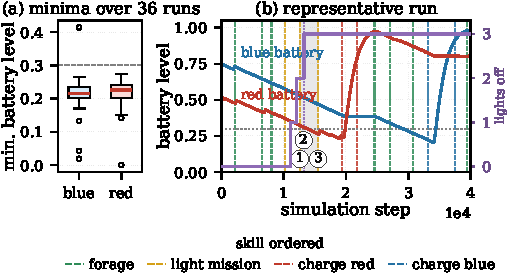
\includegraphics[width=0.52\linewidth]{figs/singlerobot.pdf}};
    \begin{scope}[
      shift={(image.south west)},
      x={($(image.south east)-(image.south west)$)},
      y={($(image.north west)-(image.south west)$)}
    ]
      % stale-decision window in panel (b): steps 12,590 -> 15,510
      \only<2->{\draw[upmred, line width=1.4pt, rounded corners=1pt]
        (0.575,0.385) rectangle (0.642,0.905);}
    \end{scope}
  \end{tikzpicture}\\[-2pt]
  % fixed-height caption box: keeps every overlay the same height
  \begin{minipage}[t][1.2cm][t]{0.92\linewidth}
  \centering
  {\footnotesize\color{upmnavy}%
    \only<1>{\textbf{34/36 runs succeeded} -- 94.4\,\%, Wilson 95\,\% CI
      $[81.8,\,98.4]$. But a few runs approach battery exhaustion.}%
    \only<2>{\textbf{Step 12{,}590 -- query issued.} Two lights off, so
      ``continue the light mission'' was \emph{correct}.}%
    \only<3>{\textbf{Step 13{,}210 -- mission already complete.} The
      running routine switched off the third light by itself.}%
    \only<4>{\textbf{Step 15{,}510 -- the answer arrives,
      $\approx$\,2{,}900 steps stale.} Correct for the state it observed,
      obsolete by the time it took effect.}%
  }
  \end{minipage}
  \note{85 s. Start with the aggregate: 94\% success, but look at the
  outliers near zero battery. Then click through the three steps -- this
  is the pedagogical case for the whole paper. Close: the decision was
  never wrong, it was late. That is what event-driven synchronisation
  removes.}
\end{frame}

% ================= Fleet success + deployment cost ===================
\begin{frame}{Scenario 2: the fleet deploys reliably -- but not cheaply}
  \vspace{-2pt}
  \centering
  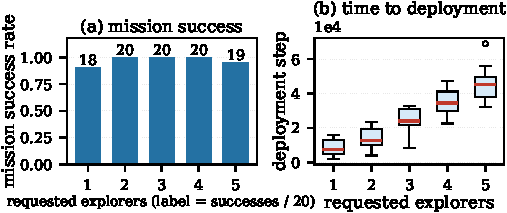
\includegraphics[width=0.62\linewidth]{figs/success.pdf}\\[4pt]
  \begin{columns}[T]
  \column{0.48\textwidth}
  \callout[upmnavy]{\footnotesize \textbf{Success.} 20/20 for fleets of
  two, three and four. Failures only at the extremes: 18/20 with one
  explorer, 19/20 with five.}
  \column{0.48\textwidth}
  \callout[upmred]{\footnotesize \textbf{Cost.} Median deployment grows
  $\sim$7{,}000 $\rightarrow$ $\sim$45{,}000 steps: the coordinator must
  \textbf{serialise recharges} before the mission can start.}
  \end{columns}
  \vspace{2pt}
  {\footnotesize\color{upmgray} No failure was caused by an LLM timeout,
  battery exhaustion or an unresolved blockage.}
  \note{70 s. Left panel: reliability is flat and high. Right panel: the
  price. Requiring n robots ready simultaneously makes it increasingly
  likely one still needs to charge. Flag that this bottleneck is
  structural, not computational.}
\end{frame}

% ================= Triangulation accuracy ============================
\begin{frame}{Cooperation buys accuracy, not just coverage}
  \vspace{-2pt}
  \centering
  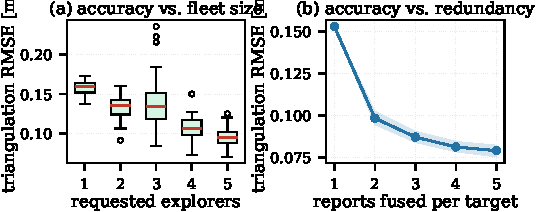
\includegraphics[width=0.62\linewidth]{figs/rmse.pdf}\\[4pt]
  \begin{columns}[T]
  \column{0.48\textwidth}
  \callout[upmnavy]{\footnotesize \textbf{By fleet size.} Median RMSE
  falls $0.16 \rightarrow 0.095$\,m from one to five explorers.
  Detection rate stays saturated at $1.0$.}
  \column{0.48\textwidth}
  \callout[upmblue]{\footnotesize \textbf{By redundancy.}
  $0.153 \rightarrow 0.098 \rightarrow 0.079$\,m for one, two and five
  reports fused. \textbf{Largest gain: one report to two.}}
  \end{columns}
  \vspace{2pt}
  {\footnotesize\color{upmgray} Robots never observe a target's true
  position -- they log \emph{their own} pose at detection.}
  \note{65 s. The clearest quantitative benefit of the multi-robot
  setting. Panel (b) isolates the mechanism: it is redundant, partially
  independent evidence about the same target, not merely more arena
  covered. Error roughly halves.}
\end{frame}

% ================= Robustness / invalid decisions ====================
\begin{frame}{Invalid decisions do not become failed missions}
  \begin{columns}[T]
  \column{0.52\textwidth}
  \vspace{-2pt}
  \footnotesize
  \begin{tabular}{@{}lcccc@{}}
    \toprule
    \textbf{\color{upmnavy}Explorers} & 1 & 3 & 5 & \textbf{total} \\
    \midrule
    Self-check contradiction & 11 & 41 & 82 & \textbf{218} \\
    Malformed JSON           &  0 &  0 &  2 & \textbf{3}  \\
    Constraint violation     &  0 &  0 &  4 & \textbf{4}  \\
    \midrule
    \textbf{All invalid}     & 11 & 41 & 88 & \textbf{225} \\
    \bottomrule
  \end{tabular}
  \vspace{6pt}
  \begin{itemize}\small
    \item Failures are \textbf{not of format} -- the prompt controls that
      well
    \item They are failures of \textbf{arithmetic consistency} over a
      longer robot list
  \end{itemize}
  \column{0.48\textwidth}
  \vspace{4pt}
  \callout[upmblue]{\footnotesize \textbf{Most invalid decisions:}
  five explorers (88) $\rightarrow$ \textbf{1 failed run}\\[2pt]
  \textbf{Fewest:} one explorer (11) $\rightarrow$ \textbf{2 failed runs}}
  \vspace{6pt}
  \callout[upmnavy]{\footnotesize An invalid decision costs \textbf{one
  deliberation cycle}, not the mission: the next query is issued from an
  updated state, and the robot waits in \texttt{stop}.}
  \end{columns}
  \note{50 s. Mission success and decision quality are different things.
  The self-check block catches almost everything. Punchline: invalid-decision
  count does not predict mission failure in this data.}
\end{frame}

% ================= Latency / cost of coordination ====================
\begin{frame}{What coordination costs}
  \begin{columns}[T]
  \column{0.54\textwidth}
  \vspace{-2pt}
  \footnotesize
  \begin{tabular}{@{}ccc@{}}
    \toprule
    \textbf{\color{upmnavy}Explorers} &
    \textbf{\color{upmnavy}Local [s]} &
    \textbf{\color{upmnavy}Central [s]} \\
    \midrule
    1 & \ \ 5.5\ \ [4.8--7.2]\ \  & 27.9 \\
    3 & 12.2 [9.0--15.7]  & 28.2 \\
    5 & 21.5 [13.5--26.4] & 35.3 \\
    \bottomrule
  \end{tabular}
  \vspace{4pt}\\
  {\scriptsize\color{upmgray} local: median [IQR] per-robot query;
  central: mean per coordination query}
  \vspace{6pt}
  \begin{itemize}\small
    \item Not only \textbf{slower} -- also \textbf{less predictable}\\[-1pt]
      {\footnotesize\color{upmgray} the interquartile range widens with
      the fleet}
  \end{itemize}
  \column{0.46\textwidth}
  \vspace{2pt}
  \callout[upmnavy]{\footnotesize \textbf{Suits:} missions whose decision
  points are \textbf{tens of seconds apart} -- exploration, inspection,
  monitoring, where a skill runs far longer than the query that selected it.}
  \vspace{4pt}
  \callout[upmred]{\footnotesize \textbf{Does not suit:} anything needing
  \textbf{sub-second re-planning} -- reactive pursuit, manipulation under
  contact.}
  \vspace{4pt}
  {\footnotesize\color{upmgray} The architecture \emph{bounds} the
  consequence of latency rather than removing it: obstacle avoidance never
  waits on a query, so a slow answer costs mission time, not integrity.}
  \end{columns}
  \note{50 s. Be honest about the numbers. The key framing is the last
  line: latency costs mission time, never safety, because the reactive
  layer is independent of any query.}
\end{frame}

\section{Conclusions}

% ================= Limitations =======================================
\begin{frame}{What this does \emph{not} yet show}
  \begin{columns}[T]
  \column{0.5\textwidth}
  \textbf{\color{upmred}Transfer gaps}
  \begin{itemize}\small
    \item \textbf{Perception:} a false positive enters the abstraction
      layer as a \emph{confident} observation
    \item \textbf{Actuation:} exact termination conditions must become
      tolerance-based; odometry drift
    \item \textbf{Communication:} blackboard assumed reliable and
      instantaneous
  \end{itemize}
  \column{0.5\textwidth}
  \textbf{\color{upmred}Evaluation gaps}
  \begin{itemize}\small
    \item \textbf{One model only} -- sensitivity to scale is open
    \item \textbf{No MRTA baseline.} A threshold or auction allocator would
      very likely deploy \emph{faster} here
    \item \textbf{Simple arena:} no clutter, colour-separable targets
  \end{itemize}
  \vspace{4pt}
  \callout[upmnavy]{\footnotesize The regime where the architecture should
  win is one where the allocation criterion is \textbf{not known in
  advance} -- and we have not yet built that scenario.}
  \end{columns}
  \note{40 s. Say this plainly; reviewers asked for it and an honest
  limitations slide buys credibility in questions. Concede the baseline
  point explicitly.}
\end{frame}

% ================= Conclusions + future work =========================
\begin{frame}{Conclusions and future work}
  \begin{columns}[T]
  \column{0.52\textwidth}
  \textbf{\color{upmnavy}Contributions}
  \begin{itemize}\small
    \item A \textbf{two-level LLM hierarchy}: central allocation +
      per-robot skill selection, over a closed catalogue
    \item \textbf{Event-driven synchronisation} removes the
      stale-decision problem structurally
    \item \textbf{94.4\,\%} success (single robot), \textbf{100\,\%} for
      fleets of two to four
    \item Localisation error \textbf{halved} as independent reports
      accumulate
  \end{itemize}
  \column{0.48\textwidth}
  \textbf{\color{upmnavy}Future work}
  \begin{itemize}\small
    \item Deployment on \textbf{physical robots}
    \item Evaluation \textbf{across model scales}
    \item Comparison against \textbf{conventional task allocation}
    \item \textbf{Distributing the coordinator}\\[-1pt]
      {\footnotesize\color{upmgray} auction-based allocation, a smaller
      model for routine bookkeeping, or partial deployment}
  \end{itemize}
  \vspace{4pt}
  \callout[upmblue]{\footnotesize Established \textbf{in simulation}:
  evidence the architecture is sound, not performance guarantees for a
  fielded system.}
  \end{columns}
  \note{55 s. Land the two contributions, then the two headline numbers,
  then be explicit that this is simulation evidence. End on the
  coordinator bottleneck as the most interesting next step.}
\end{frame}

% ================= Slide: Thanks =================
\begin{frame}[plain,noframenumbering]
  \vspace{0.4cm}
  {\color{upmblue}\rule{\textwidth}{2.2pt}}\\[10pt]
  \begin{center}
  {\Huge\bfseries\color{upmnavy} Thank you}\\[4pt]
  {\color{upmred}\rule{2cm}{2pt}}\\[6pt]
  {\Large\color{upmnavy} Questions?}
  \end{center}
  \vspace{0.3cm}
  \begin{columns}[T]
  \column{0.45\textwidth}
  \textbf{\color{upmnavy}Contact}\\[2pt]
  \small
  \presenterName\\
  ETSI Telecomunicaci\'on, UPM\\
  \texttt{\presenterEmail}\\
  \texttt{\presenterWebsite}
  \column{0.55\textwidth}
  \textbf{\color{upmnavy}Acknowledgments}\\[2pt]
  \scriptsize
  Supported by Grant PID2023-146540OB-C42 funded by
  MCIN/AEI/10.13039/501100011033, and partially by the European Commission
  within the SMAUG project (EU Horizon Europe Grant Agreement 10112129)
  and the AURICA project (RP2609560188).
  \end{columns}
  \vspace{0.3cm}
  {\color{upmblue}\rule{\textwidth}{0.5pt}}\\[4pt]
  \vspace{0.2cm}
  \begin{center}
    \logoRow
  \end{center}
  \note{20 s. Thank the audience and the funders, invite questions.}
\end{frame}

\end{document}
